\chapter{Regression \label{chapter:regression}}

Classification is a form of supervised learning in which the outcome is a category. \textbf{Regression}\index{regression} is another form of supervised learning in which the outcome is a numeric value. For example, it may be a lab value, physical characteristic (height, weight, etc.), or numeric measurement (e.g. oxygen saturation).

%%%%%%%%%%%%%%%%%%%%%%%%%%%%%%%%%%%%%%%%%%%%%%%%%%%%%%%%%%%%%%%%%%%%%%%%%%%%%%%%%%%%%%

\section{Visualizing the Regression Problem \label{section:visualizingreg}}

Let's consider the same setup from Section~\ref{section:visualizingclass} but this time with a quantitative outcome: a ``recurrence biomarker'' that indicates the likelihood of recurrence of disease.

Again, we have data on two predictors: a disease severity score ($x_1$), which characterizes the severity of the illness for which the patient was originally treated, and a social determinants score ($x_2$), which characterizes a patient's socioeconomic status. We have measurements of $x_1$ and $x_2$ on the same $200$ patients as in Section~\ref{section:visualizingclass}. 

\begin{center}
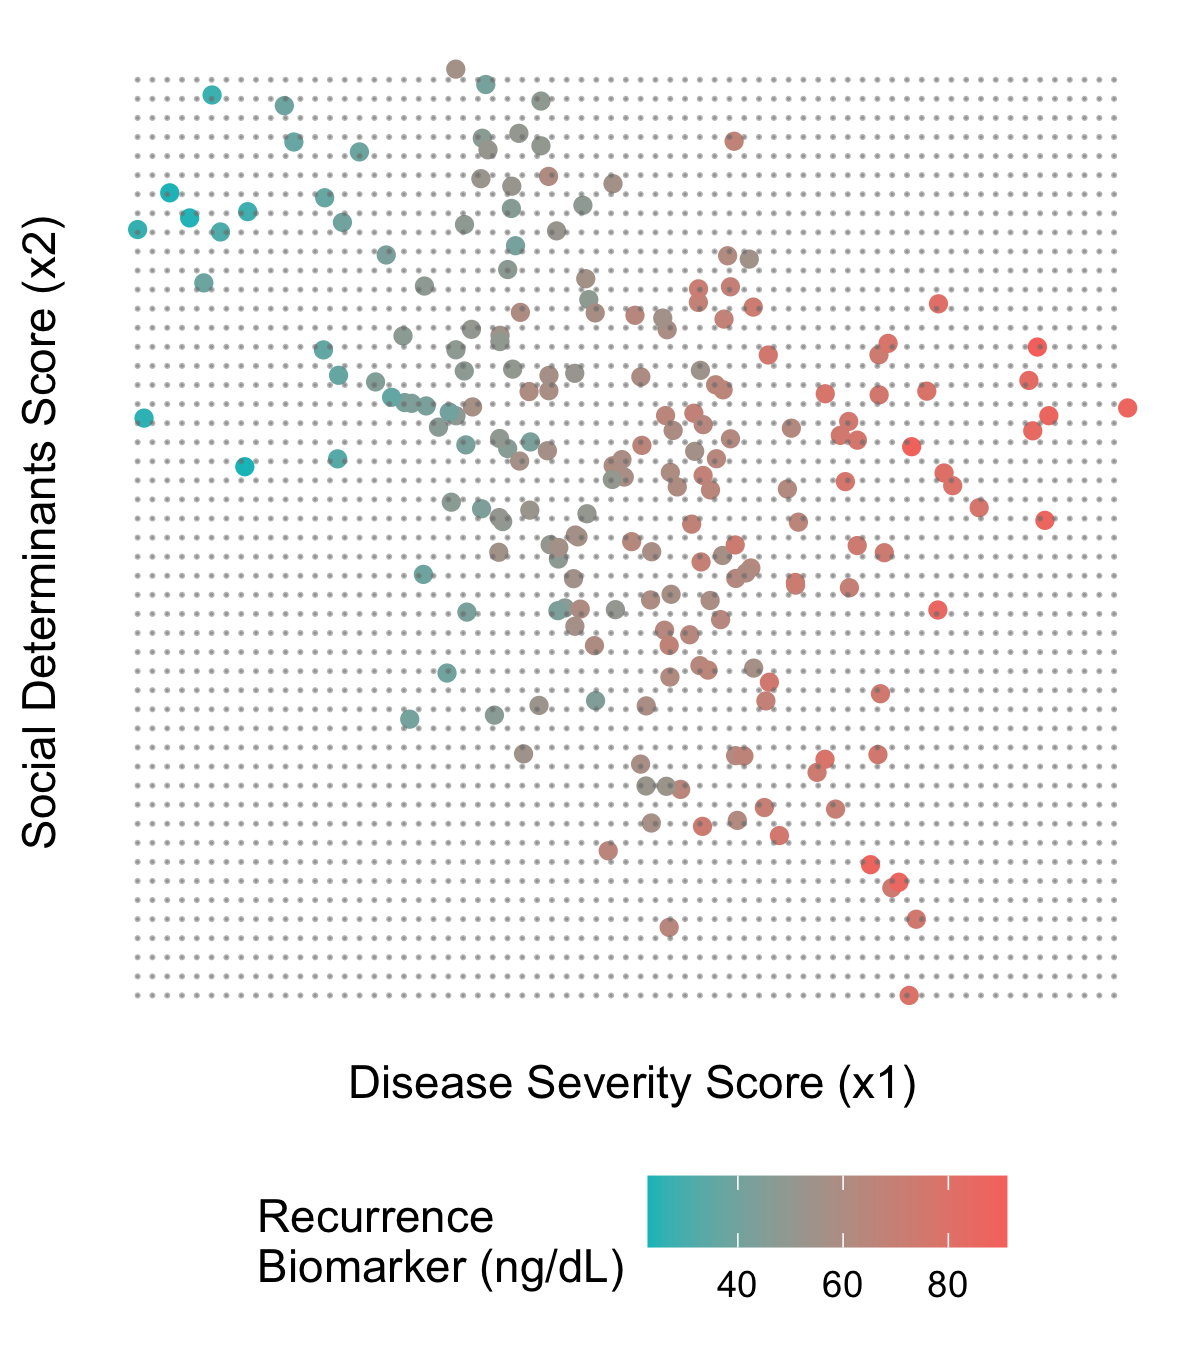
\includegraphics[width=0.7\textwidth]{img/esl-reg-just-data.png}
\end{center}

This is a plot of the data in a single plane. The color represents the value of the recurrence biomarker -- the height of the point above the plane. The goal of regression is to predict the value of the biomarker ($y$) based on the values of the two predictors, $x_1$ and $x_2$.
\vspace{5mm} 

\begin{question}{}
Just looking at the two predictors, which one appears to more highly influence the value of the recurrence biomarker? Why?
\end{question}
\vspace{2mm}

\begin{question}{}
Think about the three algorithms we discussed in Chapter~\ref{chapter:classification}. Now think about our new task, which is to predict the \emph{numeric value} of the recurrence biomarker as a function of the two predictors, $x_1$ and $x_2$. 
\begin{itemize}
\item How might you adapt KNN to deal with this problem?
\item How might you adapt a decision tree to deal with this problem?
\item How might you adapt logistic regression to deal with this problem? You'll have to ``break the algorithm'' a bit more this time.  
\end{itemize}
\end{question}

%%%%%%%%%%%%%%%%%%%%%%%%%%%%%%%%%%%%%%%%%%%%%%%%%%%%%%%%%%%%%%%%%%%%%%%%%%%%%%%%%%%%%%

\section{Three Regression Algorithms}

\subsection{K Nearest Neighbors (KNN)}

Regression using KNN works very similarly to KNN for classification. In classification, we allow the nearest $K$ points to vote on the label of a new test point. In regression, we interpolate between the values of the surrounding points to come up with the value of $y$ for a test point. Typically this is done just by averaging the $y$ values of the nearest $K$ points, but you can also do something more sophisticated, like weight their contributions by distance to the test point. 

Here is a \textbf{contour plot} of the regression surface produced by KNN ($K=15$) for our example:

\begin{center}
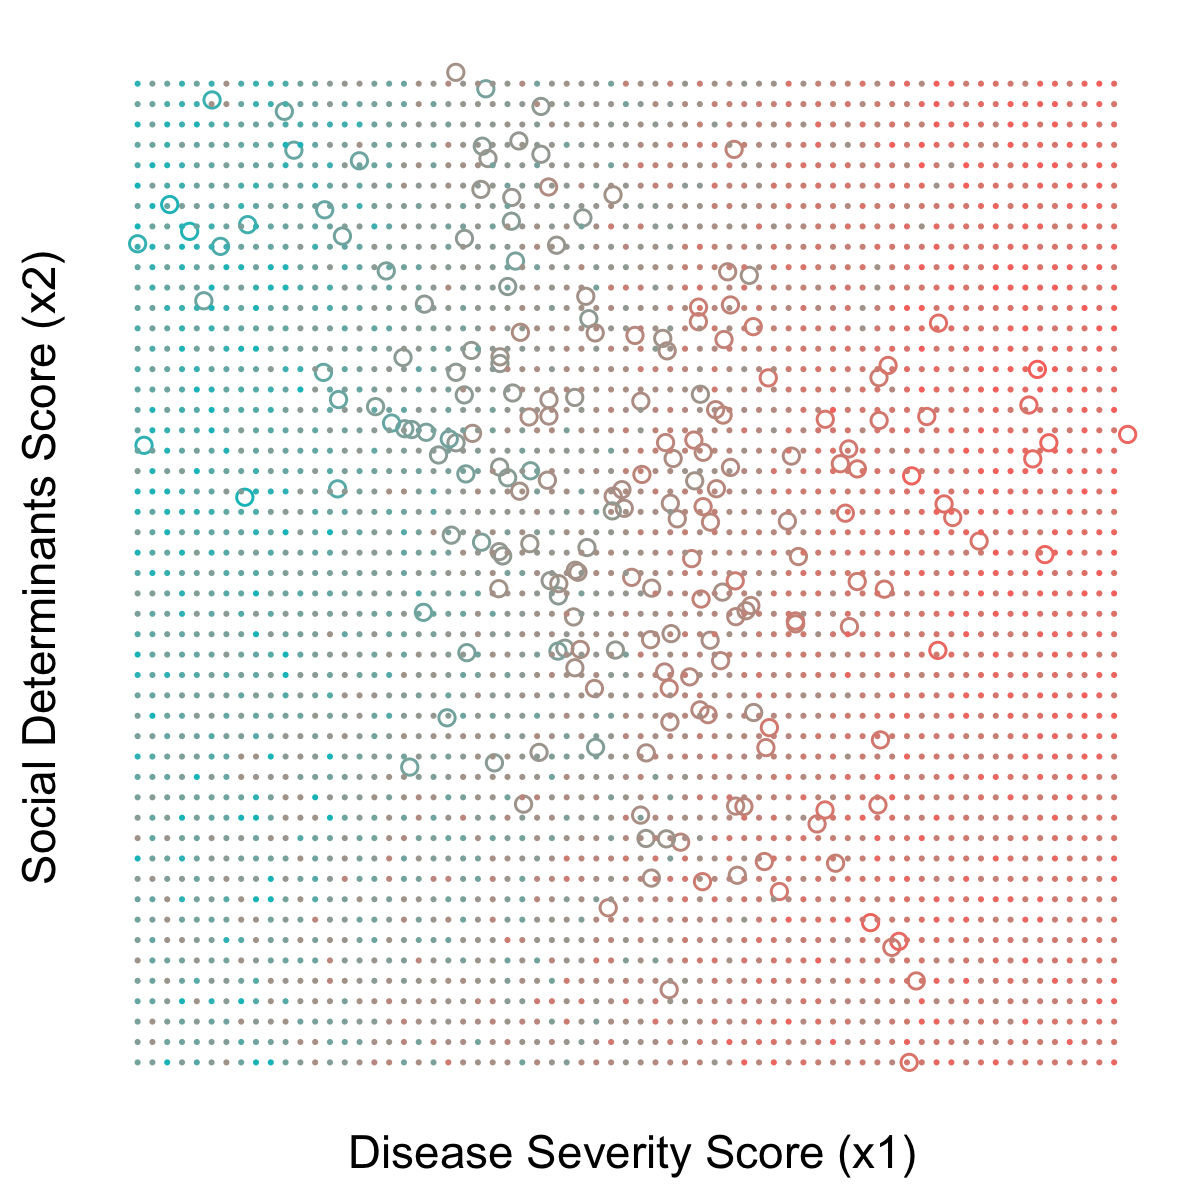
\includegraphics[width=0.7\textwidth]{img/esl-reg-knn-15.png}
\end{center}

\noindent The contours are at the 25th, 50th, and 75th percentiles of height of the regression surface. Basically this is a topographical map. Its construction is identical to the classification boundaries I drew in Chapter~\ref{chapter:classification}; it's just that instead of a single boundary, I've drawn several contours at different heights. This looks like a bit of a mess, but at the same time, the algorithm is able to capture arbitrarily complex relationships between $x_1$, $x_2$, and $y$ that can be missed by other regression algorithms.  

\subsection{Decision Tree}

In Chapter~\ref{chapter:decisiontrees}, we built a decision tree for an example in which the outcome in question was binary: yes/no. But what if the outcome is numeric? In that case, we can use \textbf{standard deviation reduction} instead of information gain to decide which variables to split on. The sample standard deviation of an outcome, $y$, is defined as:
$$ S(Y) = \sqrt{\frac{\sum_i(y^{(i)} - \overline{y})^2}{n-1}} $$
where $\overline{y}$ is the overall mean of the outcome. The procedure is identical to the ID3 algorithm (see Chapter~\ref{chapter:decisiontrees}) except you use conditional standard deviation instead of information gain to decide on features. We define
$$ S(Y, X) = \sum_{x \in \text{Values(X)}} \frac{|Y(X=x)|}{|Y|}~ S(Y(X=x)) $$
and at each current leaf node, we split on the variable where the reduction in standard deviation, $S(Y) - S(Y,X)$, is the highest.

For example, imagine you had a dataset similar in structure to our example, but instead of two real-valued predictors, you have two binary predictors, $x_1$ and $x_2$. The decision tree algorithm could choose either one of them to split on first. Here are the distributions of outcome values associated with $x_1$ and $x_2$. 

\begin{center}
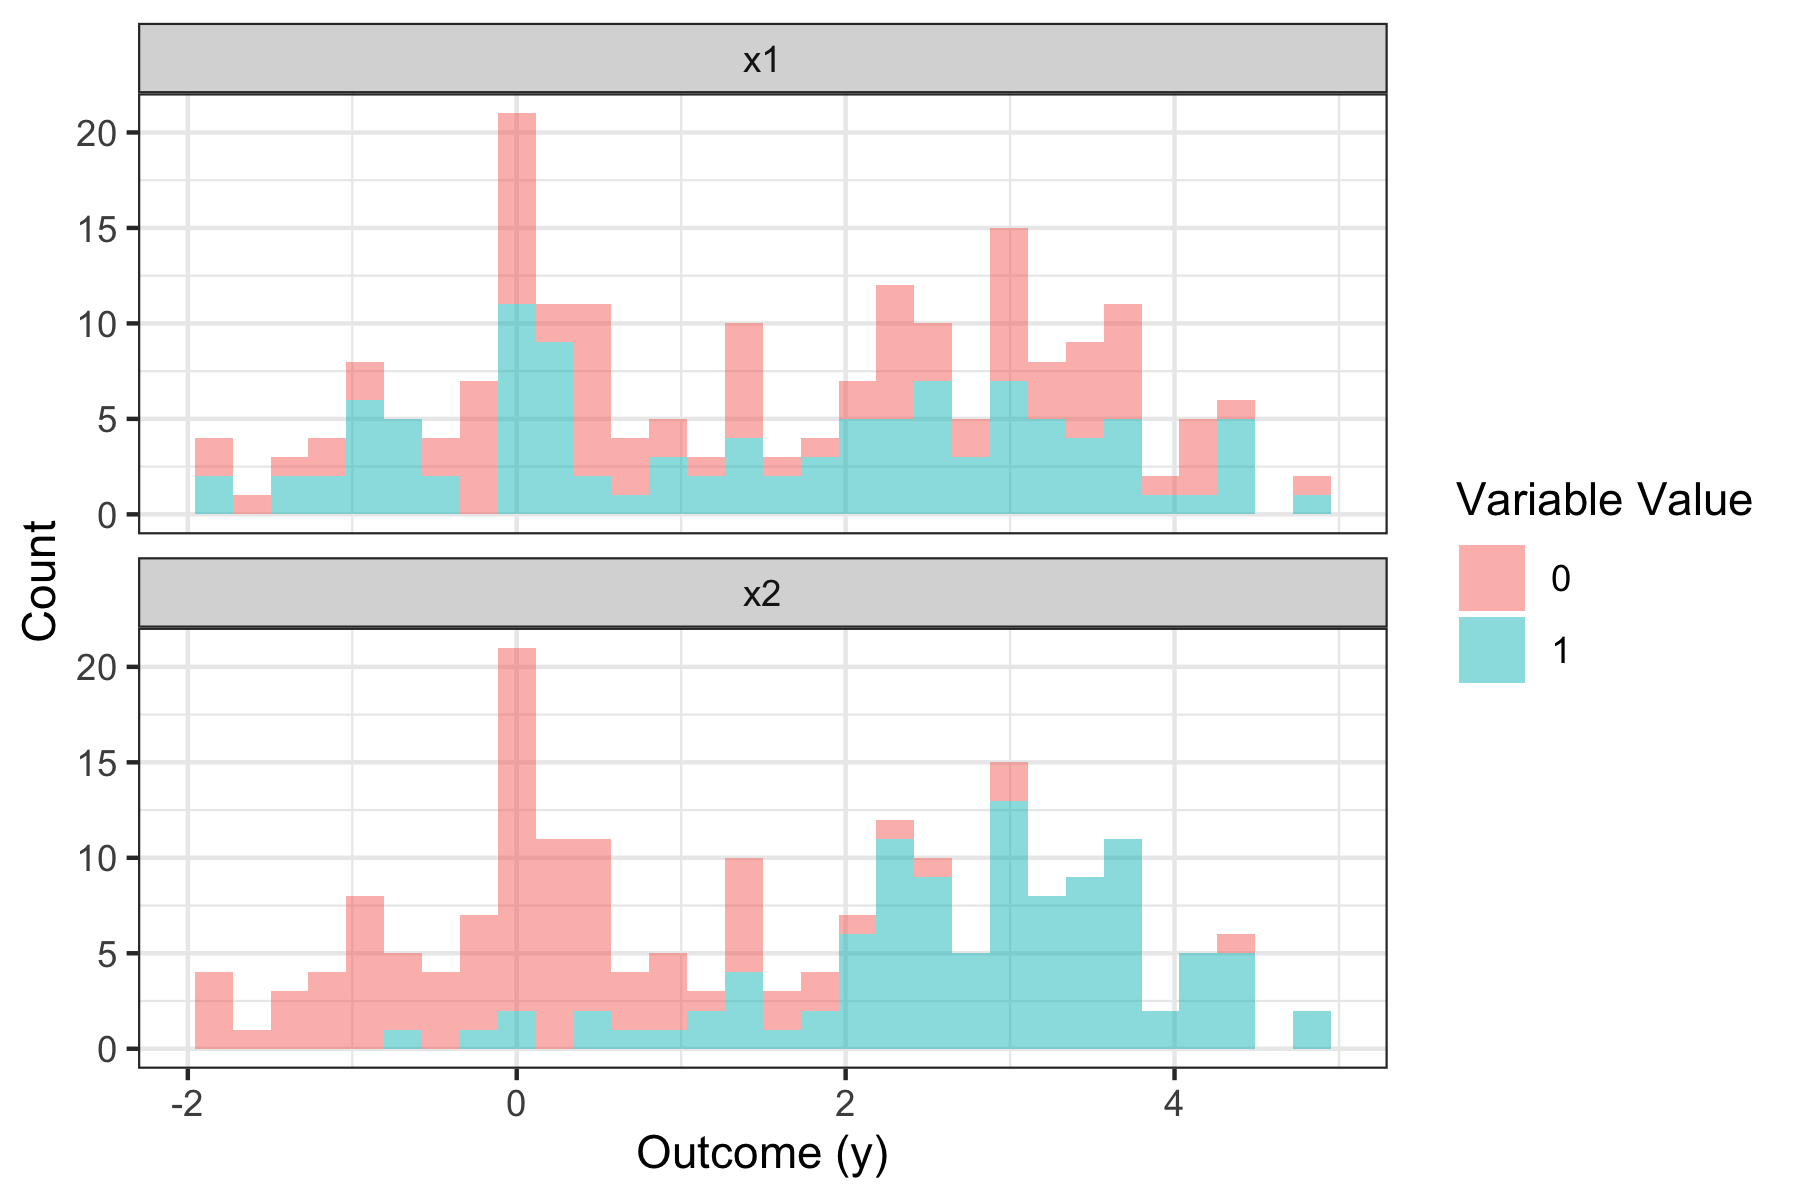
\includegraphics[width=0.9\textwidth]{img/esl-reg-decision-tree-varsplit.png}
\end{center}

\begin{question}{}
Which of these two variables, $x_1$ or $x_2$, would make the most sense for a decision tree to split on? What would such a split look like and what would the output value of the tree (the predicted value of $y$) be for each side of the split?
\end{question}

The predicted biomarker values for a decision tree trained on this dataset (created using the \texttt{rpart} package in R with default parameters) are shown here:

\begin{center}
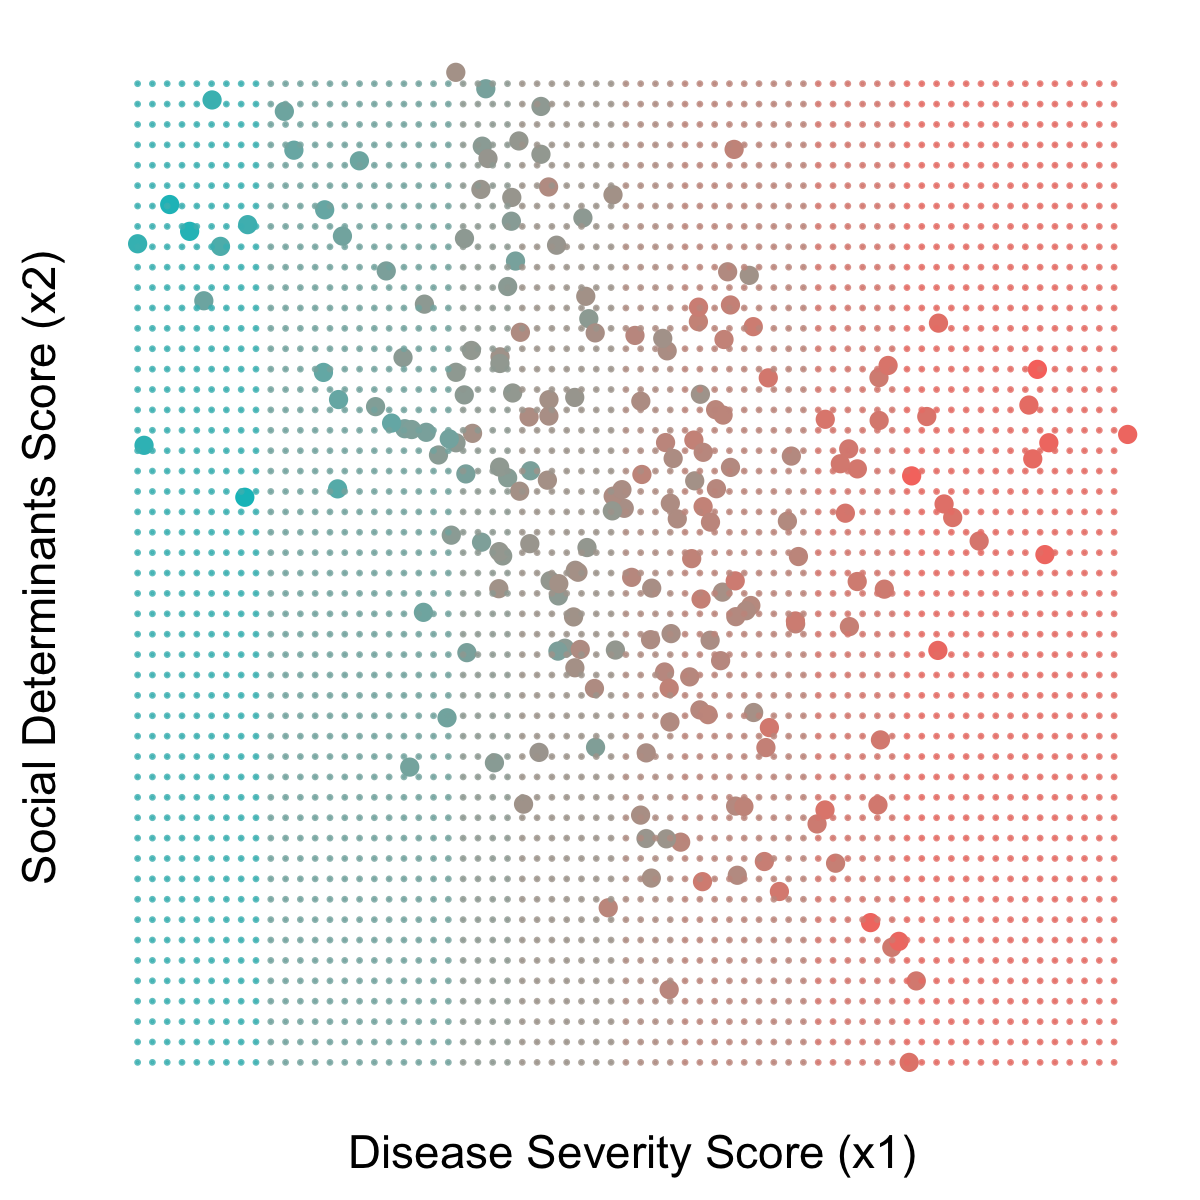
\includegraphics[width=0.7\textwidth]{img/esl-reg-decision-tree.png}
\end{center}

\subsection{Linear Regression}

% TODO

\begin{center}
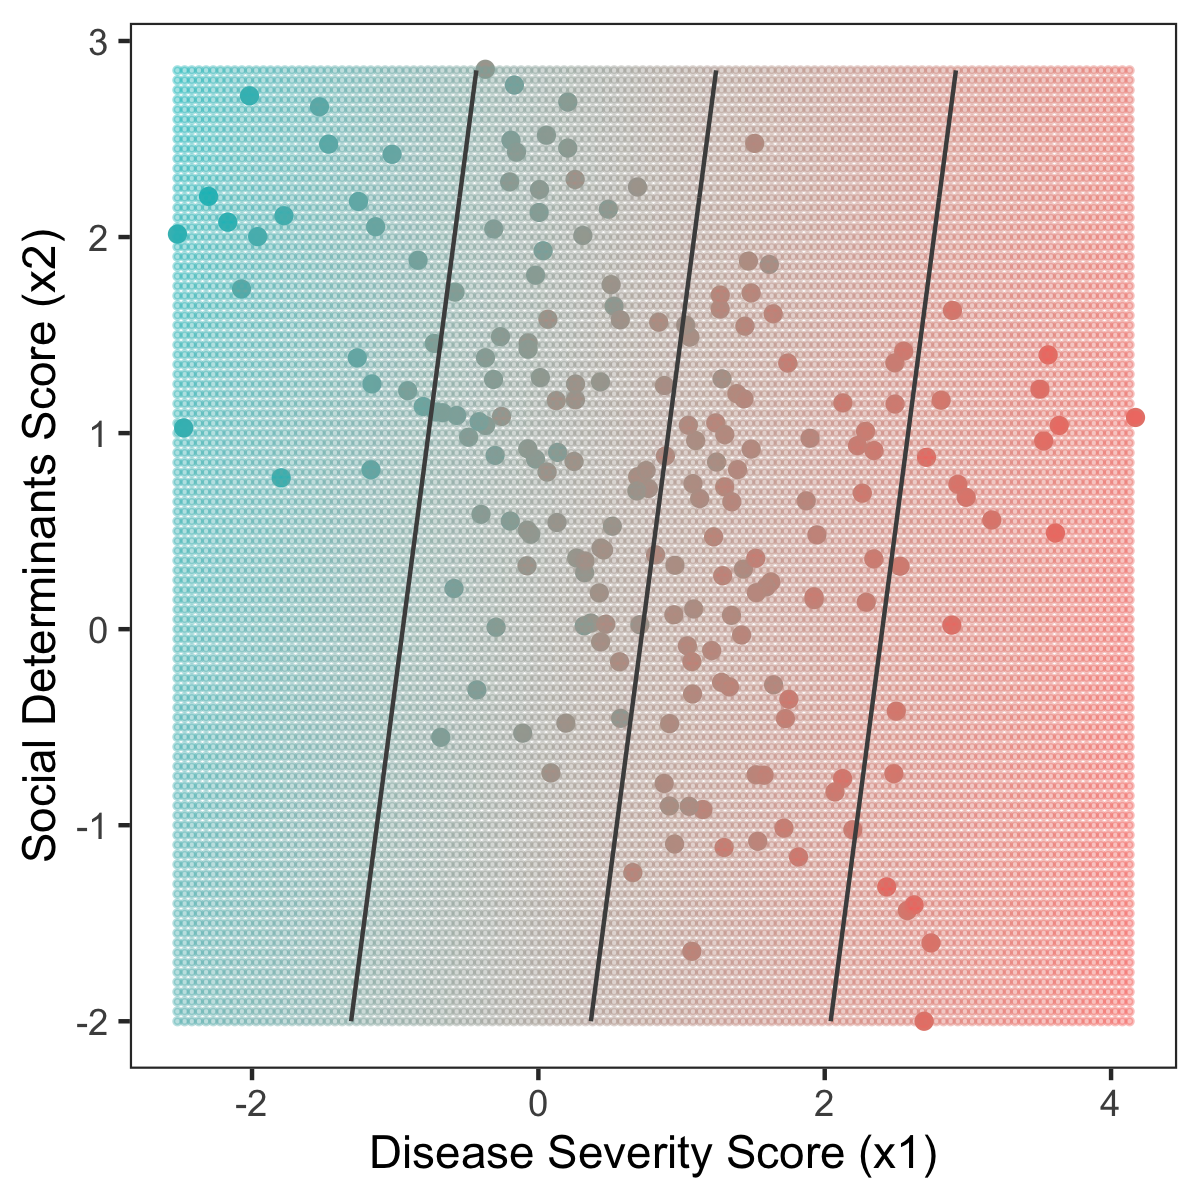
\includegraphics[width=0.7\textwidth]{img/esl-reg-linear.png}
\end{center}

\begin{question}{}
What are the advantages and disadvantages of each regression algorithm?
\end{question}

